\documentclass[dvipdfmx]{jsarticle}
\setcounter{section}{2}
\setcounter{subsection}{3}
\usepackage{xr}
\externaldocument{2.1.1}
\externaldocument{2.1.2}
\externaldocument{2.1.5}
\externaldocument{2.2.1}
\externaldocument{2.2.2}
\externaldocument{2.2.3}
\usepackage{amsmath,amsfonts,amssymb,array,comment,mathtools,url,docmute}
\usepackage{longtable,booktabs,dcolumn,tabularx,mathtools,multirow,colortbl,xcolor}
\usepackage[dvipdfmx]{graphics}
\usepackage{bmpsize}
\usepackage{amsthm}
\usepackage{enumitem}
\setlistdepth{20}
\renewlist{itemize}{itemize}{20}
\setlist[itemize]{label=•}
\renewlist{enumerate}{enumerate}{20}
\setlist[enumerate]{label=\arabic*.}
\setcounter{MaxMatrixCols}{20}
\setcounter{tocdepth}{3}
\newcommand{\rotin}{\text{\rotatebox[origin=c]{90}{$\in $}}}
\newcommand{\amap}[6]{\text{\raisebox{-0.7cm}{\begin{tikzpicture} 
  \node (a) at (0, 1) {$\textstyle{#2}$};
  \node (b) at (#6, 1) {$\textstyle{#3}$};
  \node (c) at (0, 0) {$\textstyle{#4}$};
  \node (d) at (#6, 0) {$\textstyle{#5}$};
  \node (x) at (0, 0.5) {$\rotin $};
  \node (x) at (#6, 0.5) {$\rotin $};
  \draw[->] (a) to node[xshift=0pt, yshift=7pt] {$\textstyle{\scriptstyle{#1}}$} (b);
  \draw[|->] (c) to node[xshift=0pt, yshift=7pt] {$\textstyle{\scriptstyle{#1}}$} (d);
\end{tikzpicture}}}}
\newcommand{\twomaps}[9]{\text{\raisebox{-0.7cm}{\begin{tikzpicture} 
  \node (a) at (0, 1) {$\textstyle{#3}$};
  \node (b) at (#9, 1) {$\textstyle{#4}$};
  \node (c) at (#9+#9, 1) {$\textstyle{#5}$};
  \node (d) at (0, 0) {$\textstyle{#6}$};
  \node (e) at (#9, 0) {$\textstyle{#7}$};
  \node (f) at (#9+#9, 0) {$\textstyle{#8}$};
  \node (x) at (0, 0.5) {$\rotin $};
  \node (x) at (#9, 0.5) {$\rotin $};
  \node (x) at (#9+#9, 0.5) {$\rotin $};
  \draw[->] (a) to node[xshift=0pt, yshift=7pt] {$\textstyle{\scriptstyle{#1}}$} (b);
  \draw[|->] (d) to node[xshift=0pt, yshift=7pt] {$\textstyle{\scriptstyle{#2}}$} (e);
  \draw[->] (b) to node[xshift=0pt, yshift=7pt] {$\textstyle{\scriptstyle{#1}}$} (c);
  \draw[|->] (e) to node[xshift=0pt, yshift=7pt] {$\textstyle{\scriptstyle{#2}}$} (f);
\end{tikzpicture}}}}
\renewcommand{\thesection}{第\arabic{section}部}
\renewcommand{\thesubsection}{\arabic{section}.\arabic{subsection}}
\renewcommand{\thesubsubsection}{\arabic{section}.\arabic{subsection}.\arabic{subsubsection}}
\everymath{\displaystyle}
\allowdisplaybreaks[4]
\usepackage{vtable}
\theoremstyle{definition}
\newtheorem{thm}{定理}[subsection]
\newtheorem*{thm*}{定理}
\newtheorem{dfn}{定義}[subsection]
\newtheorem*{dfn*}{定義}
\newtheorem{axs}[dfn]{公理}
\newtheorem*{axs*}{公理}
\renewcommand{\headfont}{\bfseries}
\makeatletter
  \renewcommand{\section}{%
    \@startsection{section}{1}{\z@}%
    {\Cvs}{\Cvs}%
    {\normalfont\huge\headfont\raggedright}}
\makeatother
\makeatletter
  \renewcommand{\subsection}{%
    \@startsection{subsection}{2}{\z@}%
    {0.5\Cvs}{0.5\Cvs}%
    {\normalfont\LARGE\headfont\raggedright}}
\makeatother
\makeatletter
  \renewcommand{\subsubsection}{%
    \@startsection{subsubsection}{3}{\z@}%
    {0.4\Cvs}{0.4\Cvs}%
    {\normalfont\Large\headfont\raggedright}}
\makeatother
\makeatletter
\renewenvironment{proof}[1][\proofname]{\par
  \pushQED{\qed}%
  \normalfont \topsep6\p@\@plus6\p@\relax
  \trivlist
  \item\relax
  {
  #1\@addpunct{.}}\hspace\labelsep\ignorespaces
}{%
  \popQED\endtrivlist\@endpefalse
}
\makeatother
\renewcommand{\proofname}{\textbf{証明}}
\usepackage{tikz,graphics}
\usepackage[dvipdfmx]{hyperref}
\usepackage{pxjahyper}
\hypersetup{
 setpagesize=false,
 bookmarks=true,
 bookmarksdepth=tocdepth,
 bookmarksnumbered=true,
 colorlinks=false,
 pdftitle={},
 pdfsubject={},
 pdfauthor={},
 pdfkeywords={}}
\begin{document}
%\hypertarget{ux5206ux89e3ux5b9aux7406}{%
\subsection{分解定理}%\label{ux5206ux89e3ux5b9aux7406}}
%\hypertarget{ux5e83ux7fa9ux306eux56faux6709ux7a7aux9593}{%
\subsubsection{広義の固有空間}%\label{ux5e83ux7fa9ux306eux56faux6709ux7a7aux9593}}
\begin{dfn}\label{広義の固有vector}
体$K$上のvector空間$V$、線形写像$f:V \rightarrow V$が与えられたとき、その線形写像$f$の固有値の1つ$\lambda$、恒等写像$I_{V}:V \rightarrow V$を用いて、$\exists l \in \mathbb{N}$に対し、$\left( \lambda I_{V} - f \right)^{l}\left( \mathbf{v} \right) = \mathbf{0}$が成り立つとき、そのvector$\mathbf{v}$をその線形写像$f$のその固有値$\lambda$に対する広義の固有vectorという。
\end{dfn}
\begin{thm}
\label{2.2.4.1}
体$K$上のvector空間$V$、線形写像$f:V \rightarrow V$が与えられたとき、恒等写像$I_{V}:V \rightarrow V$を用いた次式のようなその線形写像$f$の1つの固有値$\lambda$に対する広義の固有vector$\mathbf{v}$全体の集合と零vectorとの和集合$\widetilde{W_{f}}(\lambda)$はそのvector空間$V$の部分空間をなす。
\begin{align*}
\widetilde{W_{f}}(\lambda) = \bigcup_{l \in \mathbb{N}} {\ker\left( \lambda I_{V} - f \right)^{l}}
\end{align*}
さらに、その固有値$\lambda$に対する固有空間$W_{f}(\lambda)$はその集合$\widetilde{W_{f}}(\lambda)$に含まれる。
\end{thm}
\begin{dfn}\label{広義の固有空間}
上の式で定義された集合$\widetilde{W_{f}}(\lambda)$をその固有値$\lambda$に対する広義の固有空間という。
\end{dfn}
\begin{proof}
体$K$上のvector空間$V$、線形写像$f:V \rightarrow V$が与えられたとき、その線形写像$f$の1つの固有値$\lambda$に対する広義の固有vector$\mathbf{v}$全体の集合と零vectorとの和集合$\widetilde{W_{f}}(\lambda)$について、恒等写像$I_{V}:V \rightarrow V$を用いた写像$\lambda I_{V} - f$も線形写像であり、線形写像同士の合成写像もまた線形写像であるから、定義と定理\ref{2.1.2.11}より恒等写像$I_{V}:V \rightarrow V$と自然数$l$を用いた集合$\ker\left( \lambda I_{V} - f \right)^{l}$はそのvector空間$V$の部分空間をなす。さらに、$\forall\mathbf{v},\mathbf{w} \in \bigcup_{l' \in \mathbb{N}} {\ker\left( \lambda I_{V} - f \right)^{l'}}\forall k,l \in K$に対し、ある自然数たち$l_{\mathbf{v}}$、$l_{\mathbf{w}}$が存在して、次式が成り立つ。
\begin{align*}
\mathbf{v} \in \ker\left( \lambda I_{V} - f \right)^{l_{\mathbf{v}}},\ \ \mathbf{w} \in \ker\left( \lambda I_{V} - f \right)^{l_{\mathbf{w}}}
\end{align*}
このとき、次のようになることから、
\begin{align*}
\left( \lambda I_{V} - f \right)^{l_{\mathbf{v}} + l_{\mathbf{w}}}\left( k\mathbf{v} + l\mathbf{w} \right) &= k\left( \lambda I_{V} - f \right)^{l_{\mathbf{v}} + l_{\mathbf{w}}}\left( \mathbf{v} \right) + l\left( \lambda I_{V} - f \right)^{l_{\mathbf{v}} + l_{\mathbf{w}}}\left( \mathbf{w} \right)\\
&= k\left( \lambda I_{V} - f \right)^{l_{\mathbf{w}}} \circ \left( \lambda I_{V} - f \right)^{l_{\mathbf{v}}}\left( \mathbf{v} \right) \\
&\quad + l\left( \lambda I_{V} - f \right)^{l_{\mathbf{v}}} \circ \left( \lambda I_{V} - f \right)^{l_{\mathbf{w}}}\left( \mathbf{w} \right)\\
&= k\left( \lambda I_{V} - f \right)^{l_{\mathbf{w}}}\left( \mathbf{0} \right) + l\left( \lambda I_{V} - f \right)^{l_{\mathbf{v}}}\left( \mathbf{0} \right) = \mathbf{0}
\end{align*}
$k\mathbf{v} + l\mathbf{w} \in \ker\left( \lambda I_{V} - f \right)^{l_{\mathbf{v}} + l_{\mathbf{w}}}$が成り立つので、$k\mathbf{v} + l\mathbf{w} \in \bigcup_{l' \in \mathbb{N}} {\ker\left( \lambda I_{V} - f \right)^{l'}}$が成り立つ。したがって、これらの和集合$\bigcup_{l' \in \mathbb{N}} {\ker\left( \lambda I_{V} - f \right)^{l'}}$もそのvector空間$V$の部分空間をなす。\par
よって、その線形写像$f$の1つの固有値$\lambda$に対する広義の固有vector$\mathbf{v}$全体の集合と零vectorとの和集合$\widetilde{W_{f}}(\lambda)$はそのvector空間$V$の部分空間をなす。
\begin{align*}
\widetilde{W_{f}}(\lambda) = \bigcup_{l \in \mathbb{N}} {\ker\left( \lambda I_{V} - f \right)^{l}}
\end{align*}\par
さらに、その固有値$\lambda$に対する固有空間$W_{f}(\lambda)$はまさしく$\ker\left( \lambda I_{V} - f \right)$に等しいので、その集合$\widetilde{W_{f}}(\lambda)$に含まれる。
\end{proof}
\begin{thm}
\label{2.2.4.2}
体$K$上のvector空間$V$、線形写像たち$f:V \rightarrow V$、$g:V \rightarrow V$が与えられたとき、$g \circ f = f \circ g$が成り立ち、$\forall\mathbf{v} \in V\exists l,m \in \mathbb{N}$に対し、$f^{l}\left( \mathbf{v} \right) = g^{m}\left( \mathbf{v} \right) = \mathbf{0}$が成り立つなら、$\exists t \in \mathbb{N}$に対し、$(f + g)^{t}\left( \mathbf{v} \right) = \mathbf{0}$が成り立つ。
\end{thm}
\begin{proof}
体$K$上のvector空間$V$、線形写像たち$f:V \rightarrow V$、$g:V \rightarrow V$が与えられたとき、$g \circ f = f \circ g$が成り立ち、$\forall\mathbf{v} \in V\exists l,m \in \mathbb{N}$に対し、$f^{l}\left( \mathbf{v} \right) = g^{m}\left( \mathbf{v} \right) = \mathbf{0}$が成り立つなら、$l + m - 1 = t$なる自然数$t$を用いて考えれば、二項定理より次のようになる。
\begin{align*}
(f + g)^{t} &= \sum_{i \in \varLambda_{t} \cup \left\{ 0 \right\}} {\frac{t!}{i!(t - i)!}f^{i} \circ g^{t - i}}\\
&= \sum_{i \in \varLambda_{t} \setminus \varLambda_{l - 1} } {\frac{t!}{i!(t - i)!}f^{i} \circ g^{t - i}} + \sum_{i \in \varLambda_{l - 1} \cup \left\{ 0 \right\} } {\frac{t!}{i!(t - i)!}f^{i} \circ g^{t - i}}\\
&= \sum_{i \in \varLambda_{t} \setminus \varLambda_{l - 1} } {\frac{t!}{i!(t - i)!}f^{i - l} \circ f^{l} \circ g^{t - i}} + \sum_{i \in \varLambda_{l - 1} \cup \left\{ 0 \right\} } {\frac{t!}{i!(t - i)!}f^{i} \circ g^{t - i - m} \circ g^{m}}\\
&= \sum_{i \in \varLambda_{t} \setminus \varLambda_{l - 1} } {\frac{t!}{i!(t - i)!}f^{i - l} \circ g^{t - i} \circ f^{l}} + \sum_{i \in \varLambda_{l - 1} \cup \left\{ 0 \right\} } {\frac{t!}{i!(t - i)!}f^{i} \circ g^{l - 1 - i} \circ g^{m}}
\end{align*}
したがって、次のようになる。
\begin{align*}
(f + g)^{t}\left( \mathbf{v} \right) &= \left( \sum_{i \in \varLambda_{t} \setminus \varLambda_{l - 1}} {\frac{t!}{i!(t - i)!}f^{i - l} \circ g^{t - i} \circ f^{l}} \right. \\
&\quad \left.+ \sum_{i \in \varLambda_{l - 1} \cup \left\{ 0 \right\}} {\frac{t!}{i!(t - i)!}f^{i} \circ g^{l - 1 - i} \circ g^{m}} \right)\left( \mathbf{v} \right)\\
&= \left( \sum_{i \in \varLambda_{t} \setminus \varLambda_{l - 1}} {\frac{t!}{i!(t - i)!}f^{i - l} \circ g^{t - i} \circ f^{l}} \right)\left( \mathbf{v} \right) \\
&\quad + \left( \sum_{i \in \varLambda_{l - 1} \cup \left\{ 0 \right\}} {\frac{t!}{i!(t - i)!}f^{i} \circ g^{l - 1 - i} \circ g^{m}} \right)\left( \mathbf{v} \right)\\
&= \sum_{i \in \varLambda_{t} \setminus \varLambda_{l - 1}} {\frac{t!}{i!(t - i)!}f^{i - l} \circ g^{t - i} \circ f^{l}\left( \mathbf{v} \right)} \\
&\quad + \sum_{i \in \varLambda_{l - 1} \cup \left\{ 0 \right\}} {\frac{t!}{i!(t - i)!}f^{i} \circ g^{l - 1 - i} \circ g^{m}\left( \mathbf{v} \right)}\\
&= \sum_{i \in \varLambda_{t} \setminus \varLambda_{l - 1}} {\frac{t!}{i!(t - i)!}f^{i - l} \circ g^{t - i}\left( f^{l}\left( \mathbf{v} \right) \right)} \\
&\quad + \sum_{i \in \varLambda_{l - 1} \cup \left\{ 0 \right\}} {\frac{t!}{i!(t - i)!}f^{i} \circ g^{l - 1 - i}\left( g^{m}\left( \mathbf{v} \right) \right)}\\
&= \sum_{i \in \varLambda_{t} \setminus \varLambda_{l - 1}} {\frac{t!}{i!(t - i)!}f^{i - l} \circ g^{t - i}\left( \mathbf{0} \right)} \\
&\quad + \sum_{i \in \varLambda_{l - 1} \cup \left\{ 0 \right\}} {\frac{t!}{i!(t - i)!}f^{i} \circ g^{l - 1 - i}\left( \mathbf{0} \right)}\\
&= \sum_{i \in \varLambda_{t} \setminus \varLambda_{l - 1}} {\frac{t!}{i!(t - i)!}\mathbf{0}} + \sum_{i \in \varLambda_{l - 1} \cup \left\{ 0 \right\}} {\frac{t!}{i!(t - i)!}\mathbf{0}} = \mathbf{0}
\end{align*}
よって、$\exists t \in \mathbb{N}$に対し、$(f + g)^{t}\left( \mathbf{v} \right) = \mathbf{0}$が成り立つ。
\end{proof}
\begin{thm}
\label{2.2.4.3}
体$K$上のvector空間$V$、線形写像$f:V \rightarrow V$が与えられたとき、$\forall m \in \mathbb{N}\forall k \in K$に対し、恒等写像$I_{V}:V \rightarrow V$を用いたその線形写像$f$の1つの固有値$\lambda$に対する広義の固有vector$\mathbf{v}$の写像$\left( kI_{V} - f \right)^{m}$による像も、$k \neq \lambda$が成り立つなら、その固有値$\lambda$に対する広義の固有vectorである。
\end{thm}
\begin{proof}
体$K$上のvector空間$V$、線形写像$f:V \rightarrow V$が与えられたとき、$\forall m \in \mathbb{N}\forall k \in K$に対し、恒等写像$I_{V}:V \rightarrow V$を用いたその線形写像$f$の1つの固有値$\lambda$に対する広義の固有vector$\mathbf{v}$の写像$\left( kI_{V} - f \right)^{m}$による像$\left( kI_{V} - f \right)^{m}\left( \mathbf{v} \right)$について、$k \neq \lambda$が成り立つなら、その写像$\left( kI_{V} - f \right)^{m}$も線形写像であることに注意すれば、$\exists l \in \mathbb{N}$に対し、$\left( \lambda I_{V} - f \right)^{l}\left( \mathbf{v} \right) = \mathbf{0}$が成り立つので、次のようになる。
\begin{align*}
\left( \lambda I_{V} - f \right)^{l}\left( \left( kI_{V} - f \right)^{m}\left( \mathbf{v} \right) \right) &= \left( \lambda I_{V} - f \right)^{l} \circ \left( kI_{V} - f \right)^{m}\left( \mathbf{v} \right)\\
&= \left( kI_{V} - f \right)^{m} \circ \left( \lambda I_{V} - f \right)^{l}\left( \mathbf{v} \right)\\
&= \left( kI_{V} - f \right)^{m}\left( \left( \lambda I_{V} - f \right)^{l}\left( \mathbf{v} \right) \right)\\
&= \left( kI_{V} - f \right)^{m}\left( \mathbf{0} \right) = \mathbf{0}
\end{align*}\par
ここで、$\left( kI_{V} - f \right)^{m}\left( \mathbf{v} \right) = \mathbf{0}$が成り立つとすれば、これらの線形写像たち$f - \lambda I_{V}$、$kI_{V} - f$の合成は交換律が成り立つので、定理\ref{2.2.4.2}より$\exists t \in \mathbb{N}$に対し、次式が成り立つ。
\begin{align*}
\left( \left( f - \lambda I_{V} \right) + \left( kI_{V} - f \right) \right)^{t}\left( \mathbf{v} \right) = \mathbf{0}
\end{align*}
一方で、次のようになることから、
\begin{align*}
\left( \left( f - \lambda I_{V} \right) + \left( kI_{V} - f \right) \right)^{t}\left( \mathbf{v} \right) &= \left( kI_{V} - \lambda I_{V} \right)^{t}\left( \mathbf{v} \right)\\
&= \left( (k - \lambda)I_{V} \right)^{t}\left( \mathbf{v} \right)\\
&= (k - \lambda)^{t}I_{V}^{t}\left( \mathbf{v} \right)\\
&= (k - \lambda)^{t}\mathbf{v}
\end{align*}
ここで、$k - \lambda \neq 0$かつ$\mathbf{v} \neq \mathbf{0}$が成り立つので、$\left( \left( f - \lambda I_{V} \right) + \left( kI_{V} - f \right) \right)^{t}\left( \mathbf{v} \right) \neq \mathbf{0}$が成り立つ。これは先ほどの定理\ref{2.2.4.2}の結果と矛盾するので、$\left( kI_{V} - f \right)^{m}\left( \mathbf{v} \right) \neq \mathbf{0}$が成り立つ。\par
よって、広義の固有vector$\mathbf{v}$の写像$\left( kI_{V} - f \right)^{m}$による像もその固有値$\lambda$に対する広義の固有vectorである。
\end{proof}
\begin{thm}
\label{2.2.4.4}
体$K$上のvector空間$V$、線形写像$f:V \rightarrow V$が与えられたとき、$i \in \varLambda_{n}$なるその線形写像$f$の互いに異なる固有値たち$\lambda_{i}$に対する広義の固有vectors$\mathbf{v}_{i}$は線形独立である。
\end{thm}
\begin{proof}
体$K$上のvector空間$V$、線形写像$f:V \rightarrow V$が与えられたとき、$i \in \varLambda_{n}$なるその線形写像$f$の互いに異なる固有値たち$\lambda_{i}$に対する広義の固有vectors$\mathbf{v}_{i}$について、$n = 1$のときは明らかであるから、$2 \leq n$とする。$n = k$のとき、$i \in \varLambda_{k}$なるその線形写像$f$の互いに異なる固有値たち$\lambda_{i}$に対する広義の固有vectors$\mathbf{v}_{i}$は線形独立であると仮定すると、$n = k + 1$のとき、$\sum_{i \in \varLambda_{k + 1}} {c_{i}\mathbf{v}_{i}} = \mathbf{0}$が成り立つとすれば、そのvector$\mathbf{v}_{k + 1}$はその固有値$\lambda_{k + 1}$に対する広義の固有vectorであるから、$\exists l \in \mathbb{N}$に対し、恒等写像$I_{V}:V \rightarrow V$を用いた$\left( \lambda_{k + 1}I_{V} - f \right)^{l}\left( \mathbf{v}_{k + 1} \right) = \mathbf{0}$が成り立つ。このとき、その写像$\left( \lambda_{k + 1}I_{V} - f \right)^{l}$は線形写像であるから、次のようになる。
\begin{align*}
\mathbf{0} &= \left( \lambda_{k + 1}I_{V} - f \right)^{l}\left( \sum_{i \in \varLambda_{k + 1}} {c_{i}\mathbf{v}_{i}} \right)\\
&= \sum_{i \in \varLambda_{k + 1}} {c_{i}\left( \lambda_{k + 1}I_{V} - f \right)^{l}\left( \mathbf{v}_{i} \right)}\\
&= \sum_{i \in \varLambda_{k}} {c_{i}\left( \lambda_{k + 1}I_{V} - f \right)^{l}\left( \mathbf{v}_{i} \right)} + c_{k + 1}\left( \lambda_{k + 1}I_{V} - f \right)^{l}\left( \mathbf{v}_{k + 1} \right)\\
&= \sum_{i \in \varLambda_{k}} {c_{i}\left( \lambda_{k + 1}I_{V} - f \right)^{l}\left( \mathbf{v}_{i} \right)} + \mathbf{0}\\
&= \sum_{i \in \varLambda_{k}} {c_{i}\left( \lambda_{k + 1}I_{V} - f \right)^{l}\left( \mathbf{v}_{i} \right)}
\end{align*}
ここで、$\forall i \in \varLambda_{k}$に対し、$\lambda_{i} \neq \lambda_{k + 1}$が成り立つので、定理\ref{2.2.4.3}よりその族$\left\{ \left( \lambda_{k + 1}I_{V} - f \right)^{l}\left( \mathbf{v}_{i} \right) \right\}_{i \in \varLambda_{k}} $もまたそれらの互いに異なる固有値たち$\lambda_{i}$に対する広義の固有vectorsでもあり、仮定より$\forall i \in \varLambda_{k}$に対し、$c_{i} = 0$が成り立つ。このとき、次のようになることから、
\begin{align*}
\sum_{i \in \varLambda_{k + 1}} {c_{i}\mathbf{v}_{i}} &= \sum_{i \in \varLambda_{k}} {c_{i}\mathbf{v}_{i}} + c_{k + 1}\mathbf{v}_{k + 1}\\
&= \mathbf{0} + c_{k + 1}\mathbf{v}_{k + 1}\\
&= c_{k + 1}\mathbf{v}_{k + 1} = \mathbf{0}
\end{align*}
$\mathbf{v}_{k + 1} \neq 0$より$c_{k + 1} = 0$が成り立つ。以上より、$i \in \varLambda_{k + 1}$なるその線形写像$f$の互いに異なる固有値たち$\lambda_{i}$に対する広義の固有vectors$\mathbf{v}_{i}$は線形独立であることになる。\par
よって、$i \in \varLambda_{n}$なるその線形写像$f$の互いに異なる固有値たち$\lambda_{i}$に対する広義の固有vectors$\mathbf{v}_{i}$は線形独立である。
\end{proof}
\begin{thm}
\label{2.2.4.5}
体$K$上のvector空間$V$、線形写像$f:V \rightarrow V$が与えられたとき、$i \in \varLambda_{n}$なるその線形写像$f$の互いに異なる固有値たち$\lambda_{i}$に対する広義の固有空間たち$\widetilde{W_{f}}\left( \lambda_{i} \right)$の和空間$\sum_{i \in \varLambda_{n}} {\widetilde{W_{f}}\left( \lambda_{i} \right)}$は直和空間$\bigoplus_{i \in \varLambda_{n}} {\widetilde{W_{f}}\left( \lambda_{i} \right)}$でもある。
\end{thm}
\begin{proof}
体$K$上のvector空間$V$、線形写像$f:V \rightarrow V$が与えられたとき、$i \in \varLambda_{n}$なるその線形写像$f$の互いに異なる固有値たち$\lambda_{i}$に対する広義の固有空間たち$\widetilde{W_{f}}\left( \lambda_{i} \right)$の和空間$\sum_{i \in \varLambda_{n}} {\widetilde{W_{f}}\left( \lambda_{i} \right)}$について、$\forall\mathbf{v},\mathbf{w} \in \sum_{i \in \varLambda_{n}} {\widetilde{W_{f}}\left( \lambda_{i} \right)}$に対し、$\mathbf{v} = \sum_{i \in \varLambda_{n}} \mathbf{v}_{i}$、$\mathbf{w} = \sum_{i \in \varLambda_{n}} \mathbf{w}_{i}$、$\mathbf{v}_{i},\mathbf{w}_{i} \in \widetilde{W_{f}}\left( \lambda_{i} \right)$とすれば、$\sum_{i \in \varLambda_{n}} \mathbf{v}_{i} = \sum_{i \in \varLambda_{n}} \mathbf{w}_{i}$が成り立つなら、次のようになり、
\begin{align*}
\mathbf{0} = \sum_{i \in \varLambda_{n}} \mathbf{v}_{i} - \sum_{i \in \varLambda_{n}} \mathbf{w}_{i} = \sum_{i \in \varLambda_{n}} \left( \mathbf{v}_{i} - \mathbf{w}_{i} \right)
\end{align*}
ここで、$\forall i \in \varLambda_{n}$に対し、$\mathbf{v}_{i} - \mathbf{w}_{i} \in \widetilde{W_{f}}\left( \lambda_{i} \right)$が成り立つことから、定理\ref{2.2.4.4}と対偶律より$\forall i \in \varLambda_{n}$に対し、$\mathbf{v}_{i} = \mathbf{w}_{i}$が成り立つ。これにより、その和空間$\sum_{i \in \varLambda_{n}} {\widetilde{W_{f}}\left( \lambda_{i} \right)}$は直和空間$\bigoplus_{i \in \varLambda_{n}} {\widetilde{W_{f}}\left( \lambda_{i} \right)}$でもある。
\end{proof}
\begin{thm}
\label{2.2.4.6}
体$K$上の有限次元vector空間$V$、線形写像たちの族$\left\{ f_{i}:V \rightarrow V \right\}_{i \in \varLambda_{s}}$が与えられたとき、次式が成り立つ。
\begin{align*}
{\mathrm{nullity}}{f_{s} \circ \cdots \circ f_{2} \circ f_{1}} \leq \sum_{i \in \varLambda_{s}} {{\mathrm{nullity}}f_{i}}
\end{align*}
\end{thm}
\begin{proof}
体$K$上の有限次元vector空間$V$、線形写像たちの族$\left\{ f_{i}:V \rightarrow V \right\}_{i \in \varLambda_{s}}$が与えられたとき、$s = 1$のときは明らかであるから、$2 \leq s$とし、$s = k$のとき、次式が成り立つと仮定しよう。
\begin{align*}
{\mathrm{nullity}}{f_{k} \circ \cdots \circ f_{2} \circ f_{1}} \leq \sum_{i \in \varLambda_{k}} {{\mathrm{nullity}}f_{i}}
\end{align*}
$s = k + 1$のとき、$f_{k} \circ \cdots \circ f_{2} \circ f_{1} = f$とおかれると、線形写像$f_{k + 1}|V(f):V(f) \rightarrow V$について、次元公式より次のようになる。
\begin{align*}
{\mathrm{rank}}f &= \dim{V(f)}\\
&= {\mathrm{rank}}{f_{k + 1}|V(f)} + {\mathrm{nullity}}{f_{k + 1}|V(f)}\\
&= \dim{V\left( f_{k + 1}|V(f) \right)} + {\mathrm{nullity}}{f_{k + 1}|V(f)}\\
&= \dim{V\left( f_{k + 1} \circ f \right)} + {\mathrm{nullity}}{f_{k + 1}|V(f)}\\
&= {\mathrm{rank}}{f_{k + 1} \circ f} + {\mathrm{nullity}}{f_{k + 1}|V(f)}
\end{align*}
また、その線形写像たち$f:V \rightarrow V$、$f_{k + 1} \circ f:V \rightarrow V$について、次元公式より次式が成り立つので、
\begin{align*}
{\mathrm{rank}}f + {\mathrm{nullity}}f = \dim V = {\mathrm{rank}}{f_{k + 1} \circ f} + {\mathrm{nullity}}{f_{k + 1} \circ f}
\end{align*}
次のようになる。
\begin{align*}
{\mathrm{nullity}}{f_{k + 1} \circ f_{k} \circ \cdots \circ f_{2} \circ f_{1}} &= {\mathrm{nullity}}{f_{k + 1} \circ f}\\
&= \dim{V\left( f_{k + 1} \circ f \right)} + \dim{\ker{f_{k + 1} \circ f}} \\
&\quad - {\mathrm{rank}}{f_{k + 1} \circ f}\\
&= {\mathrm{rank}}f + {\mathrm{nullity}}f - {\mathrm{rank}}{f_{k + 1} \circ f}\\
&= {\mathrm{rank}}{f_{k + 1} \circ f} + {\mathrm{nullity}}{f_{k + 1}|V(f)} \\
&\quad + {\mathrm{nullity}}f - {\mathrm{rank}}{f_{k + 1} \circ f}\\
&= {\mathrm{nullity}}f + {\mathrm{nullity}}{f_{k + 1}|V(f)}\\
&= {\mathrm{nullity}}f + \dim{\ker{f_{k + 1}|V(f)}}
\end{align*}
ここで、$\forall\mathbf{v} \in V$に対し、$\mathbf{v} \in \ker{f_{k + 1}|V(f)}$が成り立つなら、$\mathbf{v} \in V(f) \subseteq V$なので、次のようになる。
\begin{align*}
f_{k + 1}|V(f)\left( \mathbf{v} \right) = f_{k + 1}\left( \mathbf{v} \right) = \mathbf{0}
\end{align*}
ゆえに、$\mathbf{v} \in \ker f_{k + 1}$が成り立ち、したがって、$\ker{f_{k + 1}|V(f)} \subseteq \ker f_{k + 1}$が成り立つことから、次のようになる。
\begin{align*}
{\mathrm{nullity}}{f_{k + 1} \circ f_{k} \circ \cdots \circ f_{2} \circ f_{1}} &\leq {\mathrm{nullity}}f + \dim{\ker f_{k + 1}}\\
&\leq \sum_{i \in \varLambda_{k}} {{\mathrm{nullity}}f_{i}} + {\mathrm{nullity}}f_{k + 1}\\
&= \sum_{i \in \varLambda_{k + 1}} {{\mathrm{nullity}}f_{i}}
\end{align*}
以上より、数学的帰納法によって線形写像たちの族$\left\{ f_{i}:V \rightarrow V \right\}_{i \in \varLambda_{s}}$が与えられたとき、次式が成り立つ。
\begin{align*}
{\mathrm{nullity}}{f_{s} \circ \cdots \circ f_{2} \circ f_{1}} \leq \sum_{i \in \varLambda_{s}} {{\mathrm{nullity}}f_{i}}
\end{align*}
\end{proof}
\begin{thm}
\label{2.2.4.7}
体$K$上の有限次元vector空間$V$、線形写像たちの族$\left\{ f_{i}:V \rightarrow V \right\}_{i \in \varLambda_{s}}$が与えられたとき、$f_{s} \circ \cdots \circ f_{2} \circ f_{1} = 0$が成り立つなら、次式が成り立つ。
\begin{align*}
n \leq \sum_{i \in \varLambda_{s}} {{\mathrm{nullity}}f_{i}}
\end{align*}
\end{thm}
\begin{proof}
体$K$上の有限次元vector空間$V$、線形写像たちの族$\left\{ f_{i}:V \rightarrow V \right\}_{i \in \varLambda_{s}}$が与えられたとき、$f_{s} \circ \cdots \circ f_{2} \circ f_{1} = 0$が成り立つなら、定理\ref{2.2.4.6}より次のようになる。
\begin{align*}
\dim{\ker{f_{s} \circ \cdots \circ f_{2} \circ f_{1}}} \leq \sum_{i \in \varLambda_{s}} {{\mathrm{nullity}}f_{i}}
\end{align*}
ここで、次元公式より次のようになるので、
\begin{align*}
\dim V &= {\mathrm{rank}}{f_{s} \circ \cdots \circ f_{2} \circ f_{1}} + {\mathrm{nullity}}{f_{s} \circ \cdots \circ f_{2} \circ f_{1}}\\
&= {\mathrm{rank}}0 + {\mathrm{nullity}}{f_{s} \circ \cdots \circ f_{2} \circ f_{1}}\\
&= 0 + {\mathrm{nullity}}{f_{s} \circ \cdots \circ f_{2} \circ f_{1}}\\
&= {\mathrm{nullity}}{f_{s} \circ \cdots \circ f_{2} \circ f_{1}}
\end{align*}
次式が成り立つ。
\begin{align*}
\dim V \leq \sum_{i \in \varLambda_{s}} {{\mathrm{nullity}}f_{i}}
\end{align*}
\end{proof}
%\hypertarget{f-ux4e0dux5909}{%
\subsubsection{$f$-不変}%\label{f-ux4e0dux5909}}
\begin{dfn}\label{f-不変の定義}
体$K$上のvector空間$V$の部分空間$W$、線形写像$f:V \rightarrow V$が与えられたとき、$V\left( f|W \right) \subseteq W$が成り立つなら、その部分空間$W$は$f$-不変であるという。
\end{dfn}
\begin{thm}
\label{2.2.4.8}
体$K$上のvector空間$V$、線形写像$f:V \rightarrow V$が与えられたとき、その値域$V(f)$と核$\ker f$は$f$-不変である。
\end{thm}
\begin{proof}
体$K$上のvector空間$V$、線形写像$f:V \rightarrow V$が与えられたとき、$V\left( f|V(f) \right) \subseteq V(f)$が成り立つかつ、$V\left( f|\ker f \right) = \left\{ \mathbf{0} \right\} \subseteq \ker f$が成り立つので、その値域$V(f)$と核$\ker f$は$f$-不変である。
\end{proof}
\begin{thm}
\label{2.2.4.9}
体$K$上のvector空間$V$、線形写像$f:V \rightarrow V$が与えられたとする。$\forall\mathbf{v} \in V$に対し、そのvector$\mathbf{v}$がその線形写像$f$の固有vectorであるならそのときに限り、$\mathbf{v} \neq \mathbf{0}$が成り立つかつ、そのvector$\mathbf{v}$から生成されるそのvector空間$V$の部分空間${\mathrm{span}}\left\{ \mathbf{v} \right\}$が$f$-不変である。
\end{thm}
\begin{proof}
体$K$上のvector空間$V$、線形写像$f:V \rightarrow V$が与えられたとする。$\forall\mathbf{v} \in V$に対し、そのvector$\mathbf{v}$がその線形写像$f$の固有vectorであるなら、$\mathbf{v} \neq \mathbf{0}$が成り立ち、さらに、その線形写像$f$のある固有値$\lambda$が存在して$f\left( \mathbf{v} \right) = \lambda\mathbf{v}$が成り立つ。このとき、$\forall k\mathbf{v} \in {\mathrm{span}}\left\{ \mathbf{v} \right\}$に対し、次のようになるので、
\begin{align*}
f\left( k\mathbf{v} \right) = \lambda k\mathbf{v} \in {\mathrm{span}}\left\{ \mathbf{v} \right\}
\end{align*}
そのvector$\mathbf{v}$から生成されるそのvector空間$V$の部分空間${\mathrm{span}}\left\{ \mathbf{v} \right\}$が$f$-不変である。\par
逆に、$\mathbf{v} \neq \mathbf{0}$が成り立つかつ、そのvector$\mathbf{v}$から生成されるそのvector空間$V$の部分空間${\mathrm{span}}\left\{ \mathbf{v} \right\}$が$f$-不変であるなら、$\forall k\mathbf{v} \in {\mathrm{span}}\left\{ \mathbf{v} \right\}$に対し、あるその体$K$の元$l$が存在して$f\left( k\mathbf{v} \right) = kf\left( \mathbf{v} \right) = l\mathbf{v}$が成り立つので、$k \neq 0$のとき、$f\left( \mathbf{v} \right) = \frac{l}{k}\mathbf{v}$が成り立つ。よって、そのvector$\mathbf{v}$がその線形写像$f$の固有vectorである。
\end{proof}
\begin{thm}
\label{2.2.4.10}
体$K$上のvector空間$V$、線形写像$f:V \rightarrow V$が与えられたとき、その線形写像$f$の1つの固有値$\lambda$に対する固有空間$W_{f}(\lambda)$、広義の固有空間$\widetilde{W_{f}}(\lambda)$は$f$-不変である。
\end{thm}
\begin{proof}
体$K$上のvector空間$V$、線形写像$f:V \rightarrow V$が与えられたとき、その線形写像$f$の1つの固有値$\lambda$に対する固有空間$W_{f}(\lambda)$、広義の固有空間$\widetilde{W_{f}}(\lambda)$について、$\forall\mathbf{v} \in W_{f}(\lambda)$に対し、$\lambda = 0$のとき、恒等写像$I_{V}:V \rightarrow V$を用いて次のようになることから、
\begin{align*}
\left( \lambda I_{V} - f \right)\left( \mathbf{v} \right) = ( - f)\left( \mathbf{v} \right) = - f\left( \mathbf{v} \right) = \mathbf{0}
\end{align*}
次のようになるので、
\begin{align*}
\left( \lambda I_{V} - f \right)\left( f\left( \mathbf{v} \right) \right) &= ( - f)\left( f\left( \mathbf{v} \right) \right)\\
&= - f \circ f\left( \mathbf{v} \right)\\
&= f\left( - f\left( \mathbf{v} \right) \right)\\
&= f\left( \mathbf{0} \right) = \mathbf{0}
\end{align*}
したがって、$f\left( \mathbf{v} \right) \in W_{f}(\lambda)$が成り立つ。$\lambda \neq 0$のとき、定理\ref{2.2.4.3}より次のようになるので、
\begin{align*}
\left( \lambda I_{V} - f \right)\left( f\left( \mathbf{v} \right) \right) &= - \left( \lambda I_{V} - f \right)\left( - f\left( \mathbf{v} \right) \right)\\
&= - \left( \lambda I_{V} - f \right)\left( ( - f)\left( \mathbf{v} \right) \right)\\
&= - \mathbf{0} = \mathbf{0}
\end{align*}
$f\left( \mathbf{v} \right) \in W_{f}(\lambda)$が成り立つ。いづれにしても、$V\left( f|W_{f}(\lambda) \right) \subseteq W_{f}(\lambda)$が成り立つので、その広義の固有空間$W_{f}(\lambda)$は$f$-不変である。\par
$\forall\mathbf{v} \in \widetilde{W_{f}}(\lambda)$に対し、$\lambda = 0$のとき、$\exists l \in \mathbb{N}$に対し、恒等写像$I_{V}:V \rightarrow V$を用いて次のようになることから、
\begin{align*}
\left( \lambda I_{V} - f \right)^{l}\left( \mathbf{v} \right) &= ( - f)^{l}\left( \mathbf{v} \right)\\
&= ( - 1)^{l}f^{l}\left( \mathbf{v} \right) = \mathbf{0}
\end{align*}
次のようになるので、
\begin{align*}
\left( \lambda I_{V} - f \right)^{l}\left( f\left( \mathbf{v} \right) \right) &= ( - f)^{l}\left( f\left( \mathbf{v} \right) \right)\\
&= ( - 1)^{l}f^{l} \circ f\left( \mathbf{v} \right)\\
&= f\left( ( - 1)^{l}f^{l}\left( \mathbf{v} \right) \right)\\
&= f\left( \mathbf{0} \right) = \mathbf{0}
\end{align*}
したがって、$f\left( \mathbf{v} \right) \in \widetilde{W_{f}}(\lambda)$が成り立つ。$\lambda \neq 0$のとき、定理\ref{2.2.4.3}より次のようになるので、
\begin{align*}
\left( \lambda I_{V} - f \right)^{l}\left( f\left( \mathbf{v} \right) \right) &= - \left( \lambda I_{V} - f \right)^{l}\left( - f\left( \mathbf{v} \right) \right)\\
&= - \left( \lambda I_{V} - f \right)^{l}\left( ( - f)\left( \mathbf{v} \right) \right)\\
&= - \mathbf{0} = \mathbf{0}
\end{align*}
$f\left( \mathbf{v} \right) \in \widetilde{W_{f}}(\lambda)$が成り立つ。いづれにしても、$V\left( f|\widetilde{W_{f}}(\lambda) \right) \subseteq \widetilde{W_{f}}(\lambda)$が成り立つので、その広義の固有空間$\widetilde{W_{f}}(\lambda)$は$f$-不変である。
\end{proof}
\begin{thm}
\label{2.2.4.11}
体$K$上のvector空間$V$が与えられたとき、多項式環$K[ X]$の多項式$\rho$の変数$X$に線形写像$f:V \rightarrow V$を代入した写像$\rho(f)$の値域$V\left( \rho(f) \right)$と核$\ker{\rho(f)}$も$f$-不変である。
\end{thm}
\begin{proof}
体$K$上のvector空間$V$が与えられたとき、$\rho = \sum_{i \in \varLambda_{r} \cup \left\{ 0 \right\}} {k_{i}X^{i}}$なる多項式環$K[ X]$の多項式$\rho$の変数$X$に線形写像$f:V \rightarrow V$を代入した写像$\rho(f)$の値域$V\left( \rho(f) \right)$と核$\ker{\rho(f)}$について、$\forall f\left( \mathbf{v} \right) \in V\left( f|V\left( \rho(f) \right) \right)$に対し、$\mathbf{v} \in V\left( \rho(f) \right)$が成り立つことから、$\exists\mathbf{w} \in V$に対し、$\rho(f)\left( \mathbf{w} \right) = \mathbf{v}$が成り立つ。このとき、定理\ref{2.1.2.10}より次のようになることから、
\begin{align*}
f\left( \mathbf{v} \right) &= f\left( \rho(f)\left( \mathbf{w} \right) \right)\\
&= f \circ \left( \sum_{i \in \varLambda_{r} \cup \left\{ 0 \right\}} {k_{i}f^{i}} \right)\left( \mathbf{w} \right)\\
&= \left( \sum_{i \in \varLambda_{r} \cup \left\{ 0 \right\}} {k_{i}f \circ f^{i}} \right)\left( \mathbf{w} \right)\\
&= \left( \sum_{i \in \varLambda_{r} \cup \left\{ 0 \right\}} {k_{i}f^{i} \circ f} \right)\left( \mathbf{w} \right)\\
&= \left( \sum_{i \in \varLambda_{r} \cup \left\{ 0 \right\}} {k_{i}f^{i}} \right) \circ f\left( \mathbf{w} \right)\\
&= \rho(f)\left( f\left( \mathbf{w} \right) \right)
\end{align*}
$f\left( \mathbf{v} \right) \in V\left( \rho(f) \right)$が成り立つ。したがって、その値域$V\left( \rho(f) \right)$は$f$-不変である。\par
一方で、$\forall f\left( \mathbf{v} \right) \in V\left( f|\ker{\rho(f)} \right)$に対し、$\mathbf{v} \in \ker{\rho(f)}$が成り立つことから、$\rho(f)\left( \mathbf{v} \right) = \mathbf{0}$が成り立つ。したがって、次のようになることから、
\begin{align*}
\rho(f)\left( f\left( \mathbf{v} \right) \right) &= \left( \sum_{i \in \varLambda_{r} \cup \left\{ 0 \right\}} {k_{i}f^{i}} \right) \circ f\left( \mathbf{v} \right)\\
&= \left( \sum_{i \in \varLambda_{r} \cup \left\{ 0 \right\}} {k_{i}f^{i} \circ f} \right)\left( \mathbf{v} \right)\\
&= \left( \sum_{i \in \varLambda_{r} \cup \left\{ 0 \right\}} {k_{i}f \circ f^{i}} \right)\left( \mathbf{v} \right)\\
&= f \circ \left( \sum_{i \in \varLambda_{r} \cup \left\{ 0 \right\}} {k_{i}f^{i}} \right)\left( \mathbf{w} \right)\\
&= f\left( \rho(f)\left( \mathbf{v} \right) \right)\\
&= f\left( \mathbf{0} \right) = \mathbf{0}
\end{align*}
$f\left( \mathbf{v} \right) \in \ker{\rho(f)}$が成り立つ。したがって、その核$\ker{\rho(f)}$は$f$-不変である。
\end{proof}
\begin{thm}
\label{2.2.4.12}
体$K$上の$n$次元vector空間$V$、線形写像$f:V \rightarrow V$が与えられたとき、$V = \bigoplus_{i \in \varLambda_{s}} W_{i}$を満たすかつ、$f$-不変な$i \in \varLambda_{s}$なるそのvector空間$V$の部分空間たち$W_{i}$の基底$\alpha_{i}$に関するその線形写像$f|W_{i}$の表現行列が$A_{i}$とおかれれば、そのvector空間$V$の基底$\left\langle \alpha_{i} \right\rangle_{i \in \varLambda_{s}}$に関するその線形写像$f$の表現行列$A$は次式のように与えられる。
\begin{align*}
A = \begin{pmatrix}
A_{1} & \  & \  & O \\
\  & A_{2} & \  & \  \\
\  & \  & \ddots & \  \\
O & \  & \  & A_{s} \\
\end{pmatrix}
\end{align*}
もちろん、その行列たち$A_{i}$の次数は$\dim W_{i}$に等しい。さらに、その線形写像$f$の固有多項式$\varPhi_{f}$は次式を満たす。
\begin{align*}
\varPhi_{f} = \prod_{i \in \varLambda_{s}} {\varPhi_{f|W_{i}}} = \varPhi_{f|W_{1}}\varPhi_{f|W_{2}}\cdots\varPhi_{f|W_{s}}
\end{align*}
\end{thm}
\begin{proof}
体$K$上の$n$次元vector空間$V$、線形写像$f:V \rightarrow V$が与えられたとき、$V = \bigoplus_{i \in \varLambda_{s}} W_{i}$を満たすかつ、$f$-不変な$i \in \varLambda_{s}$なるそのvector空間$V$の部分空間たち$W_{i}$の基底$\alpha_{i}$に関するその線形写像$f|W_{i}$の表現行列が$A_{i}$とおかれれば、$\forall\mathbf{v} \in K^{n}$に対し、$\left\langle \alpha_{i} \right\rangle_{i \in \varLambda_{s}} = \alpha$とおくと、その基底$\alpha$についてのその線形写像$f$の表現行列$[ f]_{\alpha}^{\alpha}$を$A = [ f]_{\alpha}^{\alpha}$とおくと、線形写像$L_{A}:K^{n} \rightarrow K^{n};\mathbf{v} \mapsto A\mathbf{v}$とその基底$\alpha$に関する基底変換における線形同型写像$\varphi_{\alpha}$を用いれば、次式が成り立つことから、
\begin{center}
  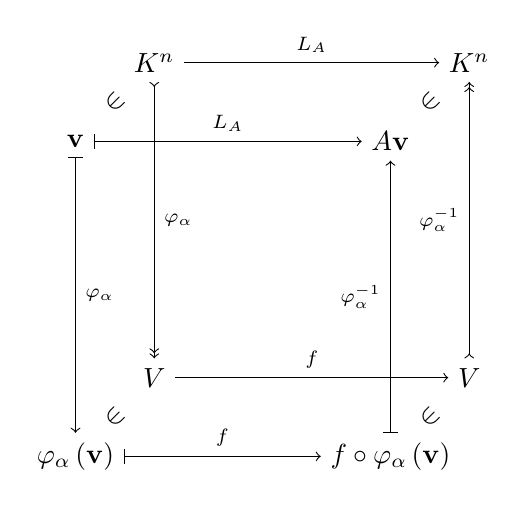
\begin{tikzpicture}[auto]

    \node (a) at (1, 5) {$K^n $};
    \node (b) at (5, 5) {$K^n $};
    \node (c) at (1, 1) {$V$};
    \node (d) at (5, 1) {$V$};
    \node (e) at (0, 4) {${\bf v} $};
    \node (f) at (4, 4) {$A{\bf v} $};
    \node (g) at (0.5, 4.5) {\rotatebox{45}{$\in $} };
    \node (h) at (4.5, 4.5) {\rotatebox{45}{$\in $} };
    \node (i) at (0, 0) {$\varphi_{\alpha } \left( {\bf v} \right) $};
    \node (j) at (4, 0) {$f\circ \varphi_{\alpha } \left( {\bf v} \right) $};
    \node (k) at (0.5, 0.5) {\rotatebox{45}{$\in $} };
    \node (l) at (4.5, 0.5) {\rotatebox{45}{$\in $} };
    
    \draw [->] (a) to node {$\scriptstyle L_A $} (b);
    \draw [|->] (e) to node {$\scriptstyle L_A $} (f);
    \draw [>->>] (d) to node {$\scriptstyle \varphi_{\alpha }^{-1} $} (b);
    \draw [|->] (j) to node {$\scriptstyle \varphi_{\alpha }^{-1} $} (f);
    \draw [->] (c) to node {$\scriptstyle f$} (d);
    \draw [|->] (i) to node {$\scriptstyle f$} (j);
    \draw [>->>] (a) to node {$\scriptstyle \varphi_{\alpha } $} (c);
    \draw [|->] (e) to node {$\scriptstyle \varphi_{\alpha } $} (i);

\end{tikzpicture}
\end{center}
$\varphi_{\alpha}\left( \mathbf{v} \right) = \bigoplus_{i \in \varLambda_{s}} \mathbf{w}_{i}$と一意的に表されることができてその基底$\alpha_{i}$に関する基底変換における線形同型写像$\varphi_{\alpha_{i}}$を用いて次のようになる。
\begin{align*}
A\mathbf{v} &= \varphi_{\alpha}^{- 1} \circ f \circ \varphi_{\alpha}\left( \mathbf{v} \right)\\
&= \varphi_{\alpha}^{- 1} \circ f\left( \bigoplus_{i \in \varLambda_{s}} \mathbf{w}_{i} \right)\\
&= \sum_{i \in \varLambda_{s}} {\varphi_{\alpha}^{- 1} \circ f\left( \mathbf{w}_{i} \right)}\\
&= \sum_{i \in \varLambda_{s}} {\varphi_{\alpha}^{- 1} \circ \varphi_{\alpha_{i}} \circ \varphi_{\alpha_{i}}^{- 1} \circ f|W_{i}\left( \mathbf{w}_{i} \right)}
\end{align*}
ここで、定理\ref{2.1.5.1}、定理\ref{2.1.5.3}より$n_{i} = \dim W_{i}$とおき線形写像$L_{A_{i}}:K^{n_{i}} \rightarrow K^{n_{i}};\mathbf{v} \mapsto A_{i}\mathbf{v}$を用いれば、次式が成り立つので、
\begin{center}
  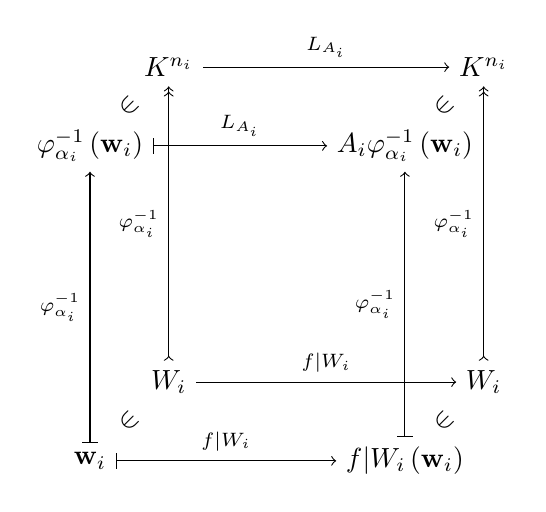
\begin{tikzpicture}[auto]

    \node (a) at (1, 5) {$K^{n_i } $};
    \node (b) at (5, 5) {$K^{n_i } $};
    \node (c) at (1, 1) {$W_i $};
    \node (d) at (5, 1) {$W_i $};
    \node (e) at (0, 4) {$\varphi_{\alpha_i }^{-1} \left( {\bf w}_i \right) $};
    \node (f) at (4, 4) {$A_i \varphi_{\alpha_i }^{-1} \left( {\bf w}_i \right) $};
    \node (g) at (0.5, 4.5) {\rotatebox{45}{$\in $} };
    \node (h) at (4.5, 4.5) {\rotatebox{45}{$\in $} };
    \node (i) at (0, 0) {${\bf w}_i $};
    \node (j) at (4, 0) {$f|W_i \left( {\bf w}_i \right) $};
    \node (k) at (0.5, 0.5) {\rotatebox{45}{$\in $} };
    \node (l) at (4.5, 0.5) {\rotatebox{45}{$\in $} };
    
    \draw [->] (a) to node {$\scriptstyle L_{A_i } $} (b);
    \draw [|->] (e) to node {$\scriptstyle L_{A_i } $} (f);
    \draw [>->>] (d) to node {$\scriptstyle \varphi_{\alpha_i }^{-1} $} (b);
    \draw [|->] (j) to node {$\scriptstyle \varphi_{\alpha_i }^{-1} $} (f);
    \draw [->] (c) to node {$\scriptstyle f|W_i $} (d);
    \draw [|->] (i) to node {$\scriptstyle f|W_i $} (j);
    \draw [>->>] (c) to node {$\scriptstyle \varphi_{\alpha_i }^{-1} $} (a);
    \draw [|->] (i) to node {$\scriptstyle \varphi_{\alpha_i }^{-1} $} (e);

\end{tikzpicture}
\end{center}
次のようになる。
\begin{align*}
A\mathbf{v} &= \sum_{i \in \varLambda_{s}} {\varphi_{\alpha}^{- 1} \circ \varphi_{\alpha_{i}} \circ L_{A_{i}} \circ \varphi_{\alpha_{i}}^{- 1}\left( \mathbf{w}_{i} \right)}\\
&= \sum_{i \in \varLambda_{s}} {\varphi_{\alpha}^{- 1} \circ \varphi_{\alpha_{i}}\left( A_{i}\varphi_{\alpha_{i}}^{- 1}\left( \mathbf{w}_{i} \right) \right)}\\
&= \begin{pmatrix}
A_{1}\varphi_{\alpha_{1}}^{- 1}\left( \mathbf{w}_{1} \right) \\
A_{2}\varphi_{\alpha_{2}}^{- 1}\left( \mathbf{w}_{2} \right) \\
 \vdots \\
A_{s}\varphi_{\alpha_{s}}^{- 1}\left( \mathbf{w}_{s} \right) \\
\end{pmatrix}\\
&= \begin{pmatrix}
A_{1} & \  & \  & O \\
\  & A_{2} & \  & \  \\
\  & \  & \ddots & \  \\
O & \  & \  & A_{s} \\
\end{pmatrix}\begin{pmatrix}
\varphi_{\alpha_{1}}^{- 1}\left( \mathbf{w}_{1} \right) \\
\varphi_{\alpha_{2}}^{- 1}\left( \mathbf{w}_{2} \right) \\
 \vdots \\
\varphi_{\alpha_{s}}^{- 1}\left( \mathbf{w}_{s} \right) \\
\end{pmatrix}
\end{align*}
ここで、次のようになることから、
\begin{align*}
\begin{pmatrix}
\varphi_{\alpha_{1}}^{- 1}\left( \mathbf{w}_{1} \right) \\
\varphi_{\alpha_{2}}^{- 1}\left( \mathbf{w}_{2} \right) \\
 \vdots \\
\varphi_{\alpha_{s}}^{- 1}\left( \mathbf{w}_{s} \right) \\
\end{pmatrix} &= \begin{pmatrix}
\varphi_{\alpha_{1}}^{- 1}\left( \mathbf{w}_{1} \right) \\
0 \\
 \vdots \\
0 \\
\end{pmatrix} + \begin{pmatrix}
0 \\
\varphi_{\alpha_{2}}^{- 1}\left( \mathbf{w}_{2} \right) \\
 \vdots \\
0 \\
\end{pmatrix} + \cdots + \begin{pmatrix}
0 \\
0 \\
 \vdots \\
\varphi_{\alpha_{s}}^{- 1}\left( \mathbf{w}_{s} \right) \\
\end{pmatrix}\\
&= \varphi_{\alpha}^{- 1}\left( \mathbf{w}_{1} \right) + \varphi_{\alpha}^{- 1}\left( \mathbf{w}_{2} \right) + \cdots + \varphi_{\alpha}^{- 1}\left( \mathbf{w}_{s} \right)\\
&= \sum_{i \in \varLambda_{s}} {\varphi_{\alpha}^{- 1}\left( \mathbf{w}_{i} \right)}\\
&= \varphi_{\alpha}^{- 1}\left( \bigoplus_{i \in \varLambda_{s}} \mathbf{w}_{i} \right)\\
&= \varphi_{\alpha}^{- 1} \circ \varphi_{\alpha}\left( \mathbf{v} \right) = \mathbf{v}
\end{align*}
よって、その表現行列$A$は次式のように与えられる。
\begin{align*}
A = \begin{pmatrix}
A_{1} & \  & \  & O \\
\  & A_{2} & \  & \  \\
\  & \  & \ddots & \  \\
O & \  & \  & A_{s} \\
\end{pmatrix}
\end{align*}
もちろん、その行列たち$A_{i}$の次数は$n_{i}$に等しい。\par
さらに、その線形写像$f$の固有多項式$\varPhi_{f}$について、次式が成り立つことから、
\begin{align*}
[ f]_{\alpha}^{\alpha} = A = \begin{pmatrix}
A_{1} & \  & \  & O \\
\  & A_{2} & \  & \  \\
\  & \  & \ddots & \  \\
O & \  & \  & A_{s} \\
\end{pmatrix},\ \ \left[ f|W_{i} \right]_{\alpha_{i}}^{\alpha_{i}} = A_{i}
\end{align*}
$\forall a \in K$に対し、恒等写像$I_{V}:V \rightarrow V$を用いれば、$n_{i}$次正方行列$I_{n_{i}}$を用いて次のようになる。
\begin{align*}
\det\left[ aI_{V} - f \right]_{\alpha}^{\alpha} &= \det\left( a\left[ I_{V} \right]_{\alpha}^{\alpha} - [ f]_{\alpha}^{\alpha} \right) = \det\left( aI_{n} - A \right)\\
&= \left| a\begin{pmatrix}
I_{n_{1}} & \  & \  & O \\
\  & I_{n_{2}} & \  & \  \\
\  & \  & \ddots & \  \\
O & \  & \  & I_{n_{s}} \\
\end{pmatrix} - \begin{pmatrix}
A_{1} & \  & \  & O \\
\  & A_{2} & \  & \  \\
\  & \  & \ddots & \  \\
O & \  & \  & A_{s} \\
\end{pmatrix} \right|\\
&= \left| \begin{matrix}
aI_{n_{1}} - A_{1} & \  & \  & O \\
\  & aI_{n_{2}} - A_{2} & \  & \  \\
\  & \  & \ddots & \  \\
O & \  & \  & aI_{n_{s}} - A_{s} \\
\end{matrix} \right|\\
&= \prod_{i \in \varLambda_{s}} {\det\left( aI_{n_{i}} - A_{i} \right)}\\
&= \prod_{i \in \varLambda_{s}} {\det\left( a\left[ I_{V}|W_{i} \right]_{\alpha_{i}}^{\alpha_{i}} - \left[ f|W_{i} \right]_{\alpha_{i}}^{\alpha_{i}} \right)}\\
&= \prod_{i \in \varLambda_{s}} {\det\left[ aI_{V}\left| W_{i} - f \right|W_{i} \right]_{\alpha_{i}}^{\alpha_{i}}}
\end{align*}
したがって、その線形写像$f$の固有多項式$\varPhi_{f}$は次式を満たす。
\begin{align*}
\varPhi_{f} = \prod_{i \in \varLambda_{s}} {\varPhi_{f|W_{i}}} = \varPhi_{f|W_{1}}\varPhi_{f|W_{2}}\cdots\varPhi_{f|W_{s}}
\end{align*}
\end{proof}
%\hypertarget{ux5206ux89e3ux5b9aux7406-1}{%
\subsubsection{分解定理}%\label{ux5206ux89e3ux5b9aux7406-1}}
\begin{thm}[分解定理]
\label{2.2.4.13}
代数的閉体$K$上の$n$次元vector空間$V$、線形写像$f:V \rightarrow V$が与えられたとき、定理\ref{2.2.3.1}よりその線形写像$f$の固有多項式$\varPhi_{f}$がその線形写像$f$の互いに異なる$s$つの固有値たち$\lambda_{i}$を用いて次式のように表されることができるので、そうするなら、
\begin{align*}
\varPhi_{f} = \prod_{i \in \varLambda_{s}} \left( X - \lambda_{i} \right)^{n_{i}},\ \ \sum_{i \in \varLambda_{s}} n_{i} = n
\end{align*}
次のことが成り立つ。
\begin{itemize}
\item
  その固有値$\lambda_{i}$に対する広義の固有空間たち$\widetilde{W_{f}}\left( \lambda_{i} \right)$すべての和空間は直和空間でこれはそのvector空間$V$に等しい、即ち、そのvector空間$V$は次式を満たす。
\begin{align*}
V = \bigoplus_{i \in \varLambda_{s}} {\widetilde{W_{f}}\left( \lambda_{i} \right)}
\end{align*}
\item
  $\forall i \in \varLambda_{s}$に対し、その固有値$\lambda_{i}$に対する広義の固有空間$\widetilde{W_{f}}\left( \lambda_{i} \right)$は恒等写像$I_{V}:V \rightarrow V$を用いて次式を満たす。
\begin{align*}
\widetilde{W_{f}}\left( \lambda_{i} \right) = \ker\left( \lambda_{i}I_{V} - f \right)^{n_{i}}
\end{align*}
\item
  $\forall i \in \varLambda_{s}$に対し、その固有値$\lambda_{i}$に対する広義の固有空間$\widetilde{W_{f}}\left( \lambda_{i} \right)$の次元は自然数$n_{i}$に等しい、即ち、次式を満たす。
\begin{align*}
\dim{\widetilde{W_{f}}\left( \lambda_{i} \right)} = {\mathrm{nullity}}\left( \lambda_{i}I_{V} - f \right)^{n_{i}} = n_{i}
\end{align*}
\end{itemize}
この定理を分解定理という。
\end{thm}
\begin{proof}
代数的閉体$K$上の$n$次元vector空間$V$、線形写像$f:V \rightarrow V$が与えられたとき、定理\ref{2.2.3.1}よりその線形写像$f$の固有多項式$\varPhi_{f}$がその線形写像$f$の互いに異なる$s$つの固有値たち$\lambda_{i}$を用いて次式のように表されることができる。
\begin{align*}
\varPhi_{f} = \prod_{i \in \varLambda_{s}} \left( X - \lambda_{i} \right)^{n_{i}},\ \ \sum_{i \in \varLambda_{s}} n_{i} = n
\end{align*}
このとき、Hamilton-Cayleyの定理より恒等写像$I_{V}:V \rightarrow V$を用いて次式が成り立ち、
\begin{align*}
\varPhi_{f}(f) = \left( \lambda_{1}I_{V} - f \right)^{n_{1}} \circ \left( \lambda_{2}I_{V} - f \right)^{n_{2}} \circ \cdots \circ \left( \lambda_{s}I_{V} - f \right)^{n_{s}} = 0
\end{align*}
さらに、$\ker\left( \lambda_{i}I_{V} - f \right)^{n_{i}} \subseteq \widetilde{W_{f}}\left( \lambda_{i} \right) \subseteq V$が成り立つので、定理\ref{2.2.1.4}、定理\ref{2.2.4.5}、定理\ref{2.2.4.7}より次のようになる。
\begin{align*}
n &\leq \sum_{i \in \varLambda_{s}} {{\mathrm{nullity}}\left( \lambda_{i}I_{V} - f \right)^{n_{i}}}\\
&= \sum_{i \in \varLambda_{s}} {\dim{\ker\left( \lambda_{i}I_{V} - f \right)^{n_{i}}}}\\
&\leq \sum_{i \in \varLambda_{s}} {\dim{\widetilde{W_{f}}\left( \lambda_{i} \right)}}\\
&= \dim{\bigoplus_{i \in \varLambda_{s}} {\widetilde{W_{f}}\left( \lambda_{i} \right)}}\\
&\leq \dim V = n
\end{align*}
したがって、$\dim{\bigoplus_{i \in \varLambda_{s}} {\widetilde{W_{f}}\left( \lambda_{i} \right)}} = n$が成り立ち、定理\ref{2.1.1.22}よりしたがって、次のことが成り立つ。
\begin{itemize}
\item
  その固有値$\lambda_{i}$に対する広義の固有空間たち$\widetilde{W_{f}}\left( \lambda_{i} \right)$すべての和空間は直和空間でこれはそのvector空間$V$に等しい、即ち、そのvector空間$V$は次式を満たす。
\begin{align*}
V = \bigoplus_{i \in \varLambda_{s}} {\widetilde{W_{f}}\left( \lambda_{i} \right)}
\end{align*}\par
\end{itemize}
また、$\exists i \in \varLambda_{s}$に対し、$\widetilde{W_{f}}\left( \lambda_{i} \right) \supset \ker\left( \lambda_{i}I_{V} - f \right)^{n_{i}}$が成り立つと仮定すれば、$\dim{\ker\left( \lambda_{i}I_{V} - f \right)^{n_{i}}} < \dim{\widetilde{W_{f}}\left( \lambda_{i} \right)}$が成り立つことから、上と同様にして、定理\ref{2.2.1.4}、定理\ref{2.2.4.5}、定理\ref{2.2.4.7}より次のようになる。
\begin{align*}
n &\leq \sum_{i \in \varLambda_{s}} {{\mathrm{nullity}}\left( \lambda_{i}I_{V} - f \right)^{n_{i}}}\\
&= \sum_{i \in \varLambda_{s}} {\dim{\ker\left( \lambda_{i}I_{V} - f \right)^{n_{i}}}}\\
&< \sum_{i \in \varLambda_{s}} {\dim{\widetilde{W_{f}}\left( \lambda_{i} \right)}}\\
&= \dim{\bigoplus_{i \in \varLambda_{s}} {\widetilde{W_{f}}\left( \lambda_{i} \right)}}\\
&= \dim V = n
\end{align*}
しかしながら、これは矛盾している。よって、次のことが成り立つ。
\begin{itemize}
\item
  $\forall i \in \varLambda_{s}$に対し、その固有値$\lambda_{i}$に対する広義の固有空間$\widetilde{W_{f}}\left( \lambda_{i} \right)$は恒等写像$I_{V}:V \rightarrow V$を用いて次式を満たす。
\begin{align*}
\widetilde{W_{f}}\left( \lambda_{i} \right) = \ker\left( \lambda_{i}I_{V} - f \right)^{n_{i}}
\end{align*}\par
\end{itemize}
また、定理\ref{2.2.4.10}より$\forall i \in \varLambda_{s}$に対し、その広義の固有空間$\widetilde{W_{f}}\left( \lambda_{i} \right)$は$f$-不変で定理\ref{2.2.4.12}より次式が成り立つ。
\begin{align*}
\varPhi_{f} = \prod_{i \in \varLambda_{s}} \varPhi_{f|\widetilde{W_{f}}\left( \lambda_{i} \right)}
\end{align*}
定理\ref{2.2.4.3}より$\forall i \in \varLambda_{s}\forall\mu_{i} \in K$に対し、$\lambda_{i} \neq \mu_{i}$が成り立つなら、$\forall\mathbf{v} \in \widetilde{W_{f}}\left( \lambda_{i} \right)$に対し、$\mathbf{v} \neq \mathbf{0}$が成り立つなら、そのvector$\left( \mu_{i}I_{V} - f|\widetilde{W_{f}}\left( \lambda_{i} \right) \right)\left( \mathbf{v} \right)$もその固有値$\lambda_{i}$に対する広義の固有vectorであるから、次式が成り立つ。
\begin{align*}
\left( \mu_{i}I_{V} - f|\widetilde{W_{f}}\left( \lambda_{i} \right) \right)\left( \mathbf{v} \right) \neq \mathbf{0}
\end{align*}
これにより、その線形写像$f|\widetilde{W_{f}}\left( \lambda_{i} \right)$はその体$K$の元$\lambda_{i}$以外に固有値をもたないことになる。したがって、次式が成り立つことになる。
\begin{align*}
\varPhi_{f|\widetilde{W_{f}}\left( \lambda_{i} \right)} = \left( X - \lambda_{i} \right)^{\dim{\widetilde{W_{f}}\left( \lambda_{i} \right)}}
\end{align*}
これにより、次式が成り立つ。
\begin{align*}
\varPhi_{f} &= \prod_{i \in \varLambda_{s}} \left( X - \lambda_{i} \right)^{n_{i}}\\
&= \prod_{i \in \varLambda_{s}} \left( X - \lambda_{i} \right)^{\dim{\widetilde{W_{f}}\left( \lambda_{i} \right)}}
\end{align*}
$\widetilde{W_{f}}\left( \lambda_{i} \right) = \ker\left( \lambda_{i}I_{V} - f \right)^{n_{i}}$よりよって、次のことが成り立つ。
\begin{itemize}
\item
  $\forall i \in \varLambda_{s}$に対し、その固有値$\lambda_{i}$に対する広義の固有空間$\widetilde{W_{f}}\left( \lambda_{i} \right)$の次元は自然数$n_{i}$に等しい、即ち、次式を満たす。
\end{itemize}
\begin{align*}
\dim{\widetilde{W_{f}}\left( \lambda_{i} \right)} = {\mathrm{nullity}}\left( \lambda_{i}I_{V} - f \right)^{n_{i}} = n_{i}
\end{align*}
\end{proof}
\begin{thm}[分解定理の拡張]
\label{2.2.4.14}
体$K$上の$n$次元vector空間$V$、線形写像$f:V \rightarrow V$が与えられたとき、$\forall\rho \in K[ X]$に対し、その多項式$\rho$の変数$X$にその線形写像$f$を代入した写像$\rho(f)$が$\rho(f) = 0$を満たすかつ、定理\ref{2.1.2.10}と素元分解の基本定理よりその多項式$\rho$は$\rho = \prod_{i \in \varLambda_{s}} {\pi_{i}}$と素元分解できるので、そうすると、これらの既約多項式たち$\pi_{i}$から定まる多項式写像$\pi_{i}$を用いて$V = \bigoplus_{i \in \varLambda_{s}} {\ker\pi_{i}}$が成り立つ。\par
この定理を分解定理の拡張という。
\end{thm}
\begin{proof}
体$K$上の$n$次元vector空間$V$、線形写像$f:V \rightarrow V$が与えられたとき、$\forall\rho \in K[ X]$に対し、その多項式$\rho$の変数$X$にその線形写像$f$を代入した写像$\rho(f)$が$\rho(f) = 0$を満たすかつ、その多項式環$K[ X]$が単項ideal整域であることと素元分解の基本定理よりその多項式$\rho$は$\rho = \prod_{i \in \varLambda_{s}} {\pi_{i}}$と素元分解できるので、そうするとする。このとき、その族$\left\{ \prod_{i' \in \varLambda_{s} \setminus \left\{ i \right\}} {\pi_{i'}} \right\}_{i \in \varLambda_{s}}$の最大公約元は単位元と同伴であることになる。したがって、その多項式環$K[ X]$が単項ideal整域であることにより次式が成り立つ。
\begin{align*}
K[ X] = \sum_{i \in \varLambda_{s}} {K[ X]\prod_{i' \in \varLambda_{s} \setminus \left\{ i \right\}} {\pi_{i'}}}
\end{align*}
これにより、その多項式環$K[ X]$の族$\left\{ \kappa_{i} \right\}_{i \in \varLambda_{s}}$が存在して、$\kappa_{i}\prod_{i' \in \varLambda_{s} \setminus \left\{ i \right\}} {\pi_{i'}} = \sigma_{i}$とおかれると、次式が成り立つ。
\begin{align*}
\overline{1} = \sum_{i \in \varLambda_{s}} {\kappa_{i}\prod_{i' \in \varLambda_{s} \setminus \left\{ i \right\}} {\pi_{i'}}} = \sum_{i \in \varLambda_{s}} {\sigma_{i}}
\end{align*}
$\forall i,j \in \varLambda_{s}$に対し、$i \neq j$のとき、$\rho = \prod_{i \in \varLambda_{s}} {\pi_{i}}$が成り立つので、次のようになる。
\begin{align*}
\sigma_{j}\sigma_{i} &= \kappa_{j}\prod_{i' \in \varLambda_{s} \setminus \left\{ j \right\}} {\pi_{i'}}\kappa_{i}\prod_{i' \in \varLambda_{s} \setminus \left\{ i \right\}} {\pi_{i'}}\\
&= \kappa_{j}\prod_{i' \in \varLambda_{s} \setminus \left\{ i,j \right\}} {\pi_{i'}}\kappa_{i}\prod_{i \in \varLambda_{s}} {\pi_{i}}\\
&= \kappa_{j}\prod_{i' \in \varLambda_{s} \setminus \left\{ i,j \right\}} {\pi_{i'}}\kappa_{i}\rho
\end{align*}\par
ここで、これらの既約多項式たち$\pi_{i}$から定まる多項式写像たちが$\pi_{i}:K \rightarrow K$と、それらの多項式たち$\kappa_{i}$から定まる多項式写像たちが$\kappa_{i}:K \rightarrow K$と、それらの多項式たち$\sigma_{i}$から定まる多項式写像たちが$\sigma_{i}:K \rightarrow K$とおかれると、次のようになるかつ、
\begin{align*}
\sigma_{j}(f) \circ \sigma_{i}(f) &= \kappa_{j}(f) \circ \prod_{i' \in \varLambda_{s} \setminus \left\{ i,j \right\}} {\pi_{i'}(f)} \circ \kappa_{i}(f) \circ \rho(f)\\
&= \kappa_{j}(f) \circ \prod_{i' \in \varLambda_{s} \setminus \left\{ i,j \right\}} {\pi_{i'}(f)} \circ \kappa_{i}(f) \circ 0 = 0
\end{align*}
恒等写像$I_{K}:K \rightarrow K$を用いて$I_{K} = \sum_{i \in \varLambda_{s}} \sigma_{i}$が成り立つことになるので、恒等写像$I_{V}:V \rightarrow V$を用いて$I_{V} = \sum_{i \in \varLambda_{s}} {\sigma_{i}(f)}$のようになる。\par
以上より、線形写像$\sigma_{i}(f):V \rightarrow V$の族$\left\{ \sigma_{i}(f) \right\}_{i \in \varLambda_{s}}$が与えられたとき、次のことを満たし、
\begin{itemize}
\item
  $\forall i,j \in \varLambda_{s}$に対し、$i \neq j$が成り立つなら、$\sigma_{j}(f) \circ \sigma_{i}(f) = 0$が成り立つ。
\item
  $i \in \varLambda_{s}$なるそれらの線形写像たち$\sigma_{i}(f)$について、$\sum_{i \in \varLambda_{s}} {\sigma_{i}(f)} = I_{V}$が成り立つ。
\end{itemize}
定理\ref{2.2.1.10}よりしたがって、次式が成り立つ。
\begin{align*}
V = \bigoplus_{i \in \varLambda_{n}} {V\left( \sigma_{i}(f) \right)}
\end{align*}\par
このとき、$\forall i \in \varLambda_{s}$に対し、次のようになることから、
\begin{align*}
\kappa_{i}\rho &= \kappa_{i}\prod_{i' \in \varLambda_{s}} {\pi_{i'}}\\
&= \kappa_{i}\prod_{i' \in \varLambda_{s} \setminus \left\{ i \right\}} {\pi_{i'}}\pi_{i}\\
&= \sigma_{i}\pi_{i}\\
&= \pi_{i}\sigma_{i}
\end{align*}
次のようになり、
\begin{align*}
\pi_{i}(f) \circ \sigma_{i}(f) &= \kappa_{i}(f) \circ \rho(f)\\
&= \kappa_{i}(f) \circ 0 = 0
\end{align*}
$\forall\mathbf{v} \in V$に対し、$\sigma_{i}(f)\left( \mathbf{v} \right) \in \ker{\pi_{i}(f)}$が成り立つので、$V\left( \sigma_{i}(f) \right) \subseteq \ker{\pi_{i}(f)}$が成り立つ。逆に、$\forall\mathbf{v} \in V$に対し、$\mathbf{v} \in \ker{\pi_{i}(f)}$が成り立つ、即ち、$\pi_{i}(f)\left( \mathbf{v} \right) = \mathbf{0}$が成り立つかつ、$\forall j \in \varLambda_{s}$に対し、$i \neq j$が成り立つなら、次のようになることから、
\begin{align*}
\sigma_{j} &= \kappa_{j}\prod_{i' \in \varLambda_{s} \setminus \left\{ j \right\}} {\pi_{i'}}\\
&= \kappa_{j}\prod_{i' \in \varLambda_{s} \setminus \left\{ i,j \right\}} {\pi_{i'}}\pi_{i}
\end{align*}
次のようになり、
\begin{align*}
\sigma_{j}(f)\left( \mathbf{v} \right) &= \kappa_{j}(f) \circ \prod_{i' \in \varLambda_{s} \setminus \left\{ i,j \right\}} {\pi_{i'}(f)} \circ \pi_{i}(f)\left( \mathbf{v} \right)\\
&= \kappa_{j}(f) \circ \prod_{i' \in \varLambda_{s} \setminus \left\{ i,j \right\}} {\pi_{i'}(f)}\left( \pi_{i}(f)\left( \mathbf{v} \right) \right)\\
&= \kappa_{j}(f) \circ \prod_{i' \in \varLambda_{s} \setminus \left\{ i,j \right\}} {\pi_{i'}(f)}\left( \mathbf{0} \right) = \mathbf{0}
\end{align*}
$\sum_{i' \in \varLambda_{s}} {\sigma_{i'}(f)} = I_{V}$よりしたがって、次のようになる。
\begin{align*}
\mathbf{v} &= \left( \sum_{i' \in \varLambda_{s}} {\sigma_{i'}(f)} \right)\left( \mathbf{v} \right)\\
&= \sum_{i' \in \varLambda_{s}} {\sigma_{i'}(f)\left( \mathbf{v} \right)}\\
&= \sum_{i' \in \varLambda_{s} \setminus \left\{ i \right\}} {\sigma_{i'}(f)\left( \mathbf{v} \right)} + \sigma_{i}(f)\left( \mathbf{v} \right)\\
&= \sum_{i' \in \varLambda_{s} \setminus \left\{ i \right\}} \mathbf{0} + \sigma_{i}(f)\left( \mathbf{v} \right)\\
&= \sigma_{i}(f)\left( \mathbf{v} \right) \in V\left( \sigma_{i}(f) \right)
\end{align*}
これにより、$\ker{\pi_{i}(f)} \subseteq V\left( \sigma_{i}(f) \right)$が成り立つ。以上より、$V\left( \sigma_{i}(f) \right) = \ker{\pi_{i}(f)}$が成り立つので、次式が成り立つ。
\begin{align*}
V = \bigoplus_{i \in \varLambda_{n}} {\ker{\pi_{i}(f)}}
\end{align*}
\end{proof}
\begin{thm}[対角化条件]
\label{2.2.4.15}
代数的閉体$K$上の$n$次元vector空間$V$、線形写像$f:V \rightarrow V$が与えられたとき、定理\ref{2.2.3.1}よりその線形写像$f$の固有多項式$\varPhi_{f}$がその線形写像$f$の互いに異なる$s$つの固有値たち$\lambda_{i}$を用いて次式のように表されることができるので、そうするなら、
\begin{align*}
\varPhi_{f} = \prod_{i \in \varLambda_{s}} \left( X - \lambda_{i} \right)^{n_{i}},\ \ \sum_{i \in \varLambda_{s}} n_{i} = n
\end{align*}
次のことは同値
\begin{itemize}
\item
  その線形写像$f$は対角化可能である。
\item
  そのvector空間$V$はその固有値$\lambda_{i}$に対する固有空間$W_{f}\left( \lambda_{i} \right)$を用いて次式が成り立つ。
\begin{align*}
V = \bigoplus_{i \in \varLambda_{s}} {W_{f}\left( \lambda_{i} \right)}
\end{align*}
\item
  その固有値$\lambda_{i}$に対する固有空間$W_{f}\left( \lambda_{i} \right)$の次元はその自然数$n_{i}$に等しい、即ち、次式が成り立つ。
\begin{align*}
\dim{W\left( \lambda_{i} \right)} = n_{i}
\end{align*}
\end{itemize}
\end{thm}
\begin{proof}
代数的閉体$K$上の$n$次元vector空間$V$、線形写像$f:V \rightarrow V$が与えられたとき、定理\ref{2.2.3.1}よりその線形写像$f$の固有多項式$\varPhi_{f}$がその線形写像$f$の互いに異なる$s$つの固有値たち$\lambda_{i}$を用いて次式のように表されることができるので、そうするなら、
\begin{align*}
\varPhi_{f} = \prod_{i \in \varLambda_{s}} \left( X - \lambda_{i} \right)^{n_{i}},\ \ \sum_{i \in \varLambda_{s}} n_{i} = n
\end{align*}
その固有値$\lambda_{i}$に対する固有空間$W_{f}\left( \lambda_{i} \right)$に属する$\dim{W_{f}\left( \lambda_{i} \right)}$つの線形独立なその線形写像$f$の固有vectorsが存在して、定理\ref{2.2.1.15}より和空間$\sum_{i \in \varLambda_{n}} {W_{f}\left( \lambda_{i} \right)}$は直和空間$\bigoplus_{i \in \varLambda_{n}} {W_{f}\left( \lambda_{i} \right)}$でもあるから、定理\ref{2.2.1.3}より次のようになり、
\begin{align*}
\dim{\sum_{i \in \varLambda_{s}} {W_{f}\left( \lambda_{i} \right)}} = \dim{\bigoplus_{i \in \varLambda_{s}} {W_{f}\left( \lambda_{i} \right)}} = \sum_{i \in \varLambda_{s}} {\dim{W_{f}\left( \lambda_{i} \right)}}
\end{align*}
したがって、そのvector空間$V$に属する$\sum_{i \in \varLambda_{s}} {\dim{W_{f}\left( \lambda_{i} \right)}}$つの線形独立な固有vectorsが存在し、さらに、これらのvectorsはその直和空間$\bigoplus_{i \in \varLambda_{s}} {W_{f}\left( \lambda_{i} \right)}$の基底でもある。ここで、定理\ref{2.2.2.12}よりその線形写像$f$は対角化可能であるならそのときに限り、そのvector空間$V$の基底をなすvectorsがいづれも固有vectorであるから、$V \subseteq \bigoplus_{i \in \varLambda_{s}} {W_{f}\left( \lambda_{i} \right)}$が成り立つことにより、したがって、次のことは同値
\begin{itemize}
\item
  その線形写像$f$は対角化可能である。
\item
  そのvector空間$V$はその固有値$\lambda_{i}$に対する固有空間$W_{f}\left( \lambda_{i} \right)$を用いて次式が成り立つ。
\begin{align*}
V = \bigoplus_{i \in \varLambda_{s}} {W_{f}\left( \lambda_{i} \right)}
\end{align*}
\end{itemize}
\par
また、分解定理より$\dim{W_{f}\left( \lambda_{i} \right)} \leq \dim{\widetilde{W_{f}}\left( \lambda_{i} \right)} = n_{i}$が成り立つので、そのvector空間$V$はその固有値$\lambda_{i}$に対する固有空間$W_{f}\left( \lambda_{i} \right)$を用いて次式が成り立つなら、
\begin{align*}
V = \bigoplus_{i \in \varLambda_{s}} {W_{f}\left( \lambda_{i} \right)}
\end{align*}
次のようになる。
\begin{align*}
n &= \dim V\\
&= \dim{\bigoplus_{i \in \varLambda_{s}} {W_{f}\left( \lambda_{i} \right)}}\\
&= \sum_{i \in \varLambda_{s}} {\dim{W_{f}\left( \lambda_{i} \right)}}\\
&\leq \sum_{i \in \varLambda_{s}} n_{i} = n
\end{align*}
したがって、$\sum_{i \in \varLambda_{s}} {\dim{W_{f}\left( \lambda_{i} \right)}} = \sum_{i \in \varLambda_{s}} n_{i}$が成り立つ。そこで、$\exists i \in \varLambda_{s}$に対し、$\dim{W_{f}\left( \lambda_{i} \right)} < n_{i}$が成り立つとすれば、次のようになるので、
\begin{align*}
\sum_{i \in \varLambda_{s}} n_{i} = \sum_{i \in \varLambda_{s}} {\dim{W_{f}\left( \lambda_{i} \right)}} < \sum_{i \in \varLambda_{s}} n_{i}
\end{align*}
矛盾している。これにより、$\dim{W_{f}\left( \lambda_{i} \right)} = n_{i}$が成り立つ。逆に、その固有値$\lambda_{i}$に対する固有空間$W_{f}\left( \lambda_{i} \right)$の次元がその自然数$n_{i}$に等しいなら、分解定理と定理\ref{2.2.1.4}より次のようになることから、
\begin{align*}
\dim V &= n = \sum_{i \in \varLambda_{s}} n_{i}\\
&= \sum_{i \in \varLambda_{s}} {\dim{W_{f}\left( \lambda_{i} \right)}}\\
&= \dim{\bigoplus_{i \in \varLambda_{s}} {W_{f}\left( \lambda_{i} \right)}}
\end{align*}
$V = \bigoplus_{i \in \varLambda_{s}} {W_{f}\left( \lambda_{i} \right)}$が成り立つ。以上より、次のことは同値である。
\begin{itemize}
\item
  そのvector空間$V$はその固有値$\lambda_{i}$に対する固有空間$W_{f}\left( \lambda_{i} \right)$を用いて次式が成り立つ。
\begin{align*}
V = \bigoplus_{i \in \varLambda_{s}} {W_{f}\left( \lambda_{i} \right)}
\end{align*}
\item
  その固有値$\lambda_{i}$に対する固有空間$W_{f}\left( \lambda_{i} \right)$の次元はその自然数$n_{i}$に等しい、即ち、次式が成り立つ。
\begin{align*}
\dim{W\left( \lambda_{i} \right)} = n_{i}
\end{align*}
\end{itemize}
\end{proof}
\begin{thebibliography}{50}
  \bibitem{1}
    松坂和夫, 線型代数入門, 岩波書店, 1980. 新装版第2刷 p247-248,265-275 ISBN978-4-00-029872-8
\end{thebibliography}
\end{document}
